\documentclass[compress]{beamer}
\usepackage{irbookslide}
\usepackage{irilmenau2}
\usepackage{tikz}
\usepackage{url}
\usepackage{ifxetex}
%\RequireXeTeX
\usepackage{fontspec} % zahteva paket euenc
\usepackage{xunicode}
\usepackage{xltxtra}
\usepackage{polyglossia}
\usepackage{minted}
\usepackage[noend]{algorithmic}
\renewcommand{\algorithmicrequire}{\textbf{Input:}}
\renewcommand{\algorithmicensure}{\textbf{Output:}}
\usepackage{xcolor,colortbl}
\usepackage{textcomp}
\usepackage{unicode-math}
%\setdefaultlanguage[script=Latin]{serbian}

\title{Stekovi}
\author{\textcopyright \ \ Goodrich, Tamassia, Goldwasser}
\institute{Katedra za informatiku, Fakultet tehničkih nauka, Univerzitet u
Novom Sadu}
\date{2014.}
\subject{Predavanja sa ASP}

\begin{document}

\frame{\titlepage}

\section[Pojam steka]{Pojam steka}
\begin{frame}[fragile]
  \frametitle{Apstraktni tipovi podataka}
  \begin{itemize}
    \item ATP je apstrakcija strukture podataka
    \item ATP definiše
    \begin{itemize}
      \item podatke koji se čuvaju
      \item operacije nad podacima
      \item uslovi kada dolazi do greške
    \end{itemize}
    \item primer: ADT koji modeluje sistem za trgovinu akcijama
    \begin{itemize}
      \item podaci: kupi/prodaj narudžbe
      \item operacije:
      \begin{itemize}
        \item order buy(stock, shares, price)
        \item order sell(stock, shares, price)
        \item void cancel(order)
      \end{itemize}
      \item greške:
      \begin{itemize}
        \item nepostojeće akcije
        \item otkazivanje narudžbe 
      \end{itemize}
    \end{itemize}
  \end{itemize}
\end{frame}

\begin{frame}[fragile]
  \frametitle{Stek ATP}
  \begin{itemize}
    \item \myred{stek} (stack) ATP čuva proizvoljne objekte
    \item ubacivanje i uklanjanje poštuje LIFO (last-in-first-out) princip
    \item primer: PEZ bombone :)
    \item glavne operacije:
    \begin{itemize}
      \item \myred{push}(object): dodaje element na vrh steka
      \item object \myred{pop}(): skida element sa vrha steka
    \end{itemize}
    \item dodatne operacije:
    \begin{itemize}
      \item object \myred{top}(): vraća najviši element bez skidanja
      \item integer \myred{len}(): vraća broj elemenata na steku
      \item boolean \myred{is\_empty}(): vraća True ako je stek prazan
    \end{itemize}
  \end{itemize}
  \begin{center}
    
\includegraphics[width=1.5cm]{asp-05-pic01.png}
  \end{center}
\end{frame}

\begin{frame}[fragile,shrink=10]
  \frametitle{Primer operacija nad stekom}
\begin{center}
\begin{tabular}{lcl}
\textbf{operacija} & \textbf{rezultat} & \textbf{sadržaj steka} \\
\hline \hline
\texttt{S.push(5)} & -- & [5] \\ 
\texttt{S.push(3)} & -- & [5,3] \\ 
\texttt{len(S)} & 2 & [5,3] \\ 
\texttt{S.pop()} & 3 & [5] \\ 
\texttt{S.is\_empty()} & False & [5] \\ 
\texttt{S.pop()} & 5 & [] \\ 
\texttt{S.is\_empty()} & True & [] \\ 
\texttt{S.pop()} & greška & [] \\ 
\texttt{S.push(7)} & -- & [7] \\ 
\texttt{S.push(9)} & -- & [7,9] \\ 
\texttt{S.top()} & 9 & [7,9] \\ 
\texttt{S.push(4)} & -- & [7,9,4] \\ 
\texttt{len(S)} & 3 & [7,9,4] \\ 
\texttt{S.pop()} & 4 & [7,9] \\ 
\texttt{S.push(6)} & -- & [7,9,6] \\ 
\texttt{S.push(8)} & -- & [7,9,6,8] \\ 
\texttt{S.pop()} & 8 & [7,9,6] \\ 
\end{tabular}
\end{center}
\end{frame}

\begin{frame}[fragile]
  \frametitle{Primene steka}
  \begin{itemize}
    \item neposredne primene
    \begin{itemize}
      \item istorija poseta stranicama u web čitaču
      \item undo sekvenca u tekst editoru
      \item lanac rekurzivnih poziva u programu
    \end{itemize}
    \item indirektne primene
    \begin{itemize}
      \item pomoćna struktura podataka za mnoge algoritme
      \item komponenta u okviru drugih struktura podataka
    \end{itemize}
  \end{itemize}
\end{frame}

\begin{frame}[fragile]
  \frametitle{Stek pomoću niza}
  \begin{itemize}
    \item implementiraćemo stek pomoću niza
    \item dodajemo elemente s leva u desno
    \item posebna promenljiva čuva indeks poslednjeg elementa
  \end{itemize}
  \begin{center}
    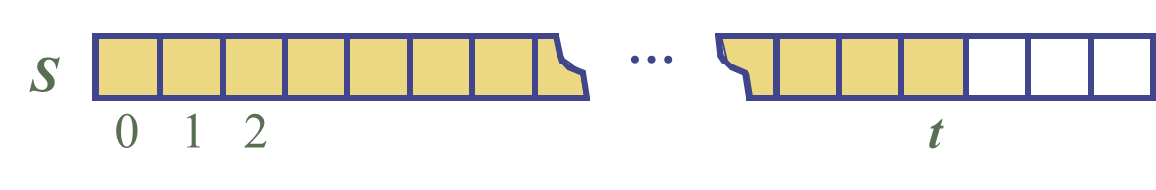
\includegraphics[width=10cm]{asp-05-pic02.png}
  \end{center}
\end{frame}

\begin{frame}[fragile]
  \frametitle{Stek pomoću niza $_2$}
  \begin{itemize}
    \item ako se niz popuni\ldots
    \item nova operacija push mora da proširi niz i iskopira sve elemente
  \end{itemize}
  \begin{center}
    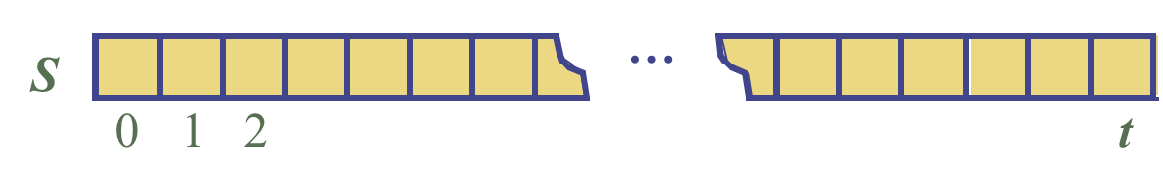
\includegraphics[width=10cm]{asp-05-pic03.png}
  \end{center}
\end{frame}

\begin{frame}[fragile]
  \frametitle{Performanse steka}
  \begin{itemize}
    \item neka je $n$ broj elemenata na steku
    \item prostor u memoriji je $O(n)$
    \item svaka operacija je $O(1)$ (amortizovano za push)
  \end{itemize}
\end{frame}

\begin{frame}[fragile,shrink=10]
  \frametitle{Implementacija steka u Pythonu}
\begin{minted}[linenos=false]{python}
class ArrayStack:
  def __init__(self):
    self._data = []
  
  def __len__(self):
    return len(self._data)
    
  def is_empty(self):
    return len(self._data) == 0
  
  def push(self, e):
    self._data.append(e)
    
  def top(self):
    if self.is_empty():
      raise Empty('stack is empty')
    return self._data[-1]
    
  def pop(self):
    if self.is_empty():
      raise Empty('stack is empty')
    return self._data.pop()
\end{minted}
\end{frame}

\section[P: Zagrade]{Primer: uparivanje zagrada}
\begin{frame}[fragile]
  \frametitle{Primer: uparivanje zagrada}
  \begin{itemize}
    \item svako (, \{, [ mora biti upareno sa ), \}, ]
    \item ispravno: ( )(( ))\{([( )])\}
    \item ispravno: ((( )(( ))\{([( )])\}
    \item neispravno: )(( ))\{([( )])\}
    \item neispravno: (\{[ ])\}
    \item neispravno: (
  \end{itemize}
\end{frame}

\begin{frame}[fragile,shrink=10]
  \frametitle{Primer: uparivanje zagrada}
\myred{ParenMatch}($X$, $n$)
\begin{algorithmic}
\REQUIRE niz $X$ od $n$ tokena, koji mogu biti zagrada, promenljiva, aritmetički operator ili broj
\ENSURE True akko su zagrade ispravno napisane
\STATE Neka je $S$ prazan stek
\FOR{$i \leftarrow 0$ \TO $n-1$}
  \IF{$X[i]$ je otvorena zagrada}
    \STATE $S$.push($X[i]$)
  \ELSIF{$X[i]$ je zatvorena zagrada}
    \IF{$S$ je prazan}
      \RETURN False \COMMENT{\myred{nema odgovarajuće otvorene zagrade}}
    \ENDIF
    \IF{$S$.pop() ne odgovara vrsti zagrade od $X[i]$}
      \RETURN False \COMMENT{\myred{pogrešna vrsta zagrade}}
    \ENDIF
  \ENDIF
\ENDFOR
\IF{$S$ je prazan}
  \RETURN True \COMMENT{\myred{svi simboli su u korektnom redosledu}}
\ELSE
  \RETURN False \COMMENT{\myred{neki simboli nemaju svoj par}}
\ENDIF
\end{algorithmic}
\end{frame}

\begin{frame}[fragile,shrink=10]
  \frametitle{Primer: uparivanje zagrada}
\begin{minted}[linenos=false]{python}
def is_matched(expr):
  """Vraća True ako se sve zagrade podudaraju."""
  lefty = '({['       # otvorene zagrade
  righty = ')}]'      # zatvorene zagrade
  S = ArrayStack()
  for c in expr:
    if c in lefty:
      S.push(c)            # stavi zagradu na stek
    elif c in righty:
      if S.is_empty():
        return False       # nema sa čime da se upari
      if righty.index(c) != lefty.index(S.pop())
        return False       # pogrešna zagrada
  return S.is_empty()      # da li su svi simboli upareni?
\end{minted}
\end{frame}

\section[P: HTML]{Primer: uparivanje zagrada}
\begin{frame}[fragile,shrink=10]
  \frametitle{Primer: uparivanje HTML tagova}
  \begin{itemize}
    \item svako \myred{\texttt{<x>}} mora biti upareno sa \myred{\texttt{</x>}}
    \item i pravilno ugnježdeno:
    \begin{itemize}
      \item \texttt{<x><y>...</y></x>} je OK
      \item \texttt{<x><y>...</x></y>} nije OK
    \end{itemize}
  \end{itemize}
  \begin{center}
    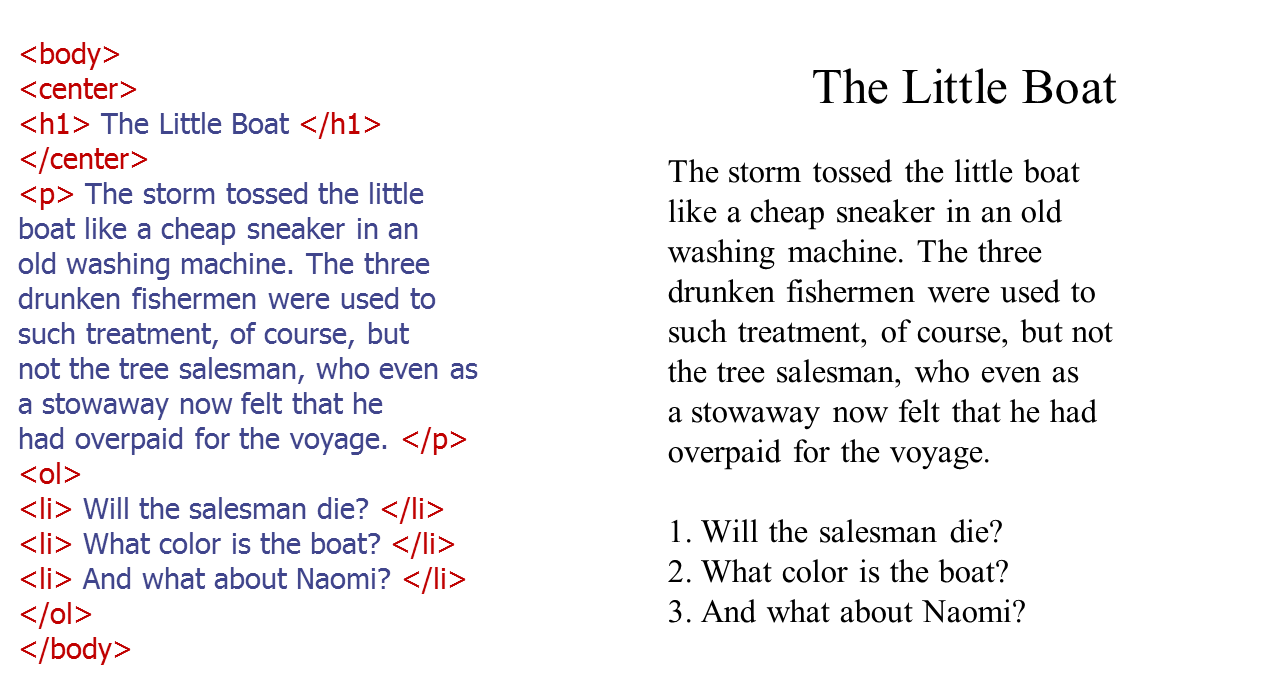
\includegraphics[width=11cm]{asp-05-pic04.png}
  \end{center}
\end{frame}

\begin{frame}[fragile,shrink=10]
  \frametitle{Primer: uparivanje HTML tagova}
\begin{minted}[linenos=false]{python}
def is_matched_html(raw):
  """Vraća True ako se HTML tagovi podudaraju."""
  S = ArrayStack()
  j = raw.find('<')             # nađi prvi '<'
  while j != -1:
    k = raw.find('>', j+1)      # nađi sledeći '>'
    if k == -1:
      return False              # neispravan tag
    tag = raw[j+1:k]            # odbaci < >
    if not tag.startswith('/'): # ovo je otvarajući tag
      S.push(tag)
    else:                       # ovo je zatvarajući tag
      if S.is_empty():
        return False            # nema svog para
      if tag[1:] != S.pop():
        return False            # nije odgovarajući par
    j = raw.find('<', k+1)      # nađi sledeći '<'
  return S.is_empty()           # svi otvarajući tagovi upareni?
\end{minted}
\end{frame}

\section[P: Izrazi]{Primer: izračunavanje aritmetičkih izraza}
\begin{frame}[fragile]
  \frametitle{Primer: izračunavanje aritmetičkih izraza}
  \begin{itemize}
    \item $14 - 3 * 2 + 7 = (14 - (3 * 2)) + 7$
    \item prioritet operatora
    \begin{itemize}
      \item * je starije od +/-
    \end{itemize}
    \item asocijativnost
    \begin{itemize}
      \item operatori istog prioriteta izračunavaju se s leva u desno
    \end{itemize}
    \item ideja:
    \begin{itemize}
      \item stavi svaki operator na stek, ali prvo skini sa steka i izračunaj 
      sve operacije višeg ili jednakog prioriteta
    \end{itemize}
  \end{itemize}
\end{frame}

\begin{frame}[fragile]
  \frametitle{Primer: izračunavanje aritmetičkih izraza}
  \begin{itemize}
    \item biće dva steka:
    \begin{itemize}
      \item $ops$ čuva operatore
      \item $vals$ čuva vrednosti
      \item koristićemo \$ kao oznaku ,,kraja ulaza`` sa najmanjim prioritetom
    \end{itemize}
  \end{itemize}
\end{frame}

\begin{frame}[fragile]
  \frametitle{Primer: izračunavanje aritmetičkih izraza}
\myred{doOp}()
\begin{algorithmic}
\STATE $x \leftarrow vals$.pop()
\STATE $y \leftarrow vals$.pop()
\STATE $op \leftarrow ops$.pop()
\STATE $vals$.push($y$ \myred{op} $x$)
\end{algorithmic}

\ %

\myred{repeatOps}(refOp)
\begin{algorithmic}
\WHILE{$vals$.size() $> 1\,\, \land$ prec($refOp$) $\leq$ prec($ops$.top())}
  \STATE doOp()
\ENDWHILE
\end{algorithmic}
\end{frame}

\begin{frame}[fragile]
  \frametitle{Primer: izračunavanje aritmetičkih izraza}
\myred{EvalExpr}()
\begin{algorithmic}
\REQUIRE lista tokena koja predstavlja aritmetički izraz
\ENSURE vrednost izraza
\WHILE{ima novi token $z$}
  \IF{$z$ je broj}
    \STATE $vals$.push($z$)
  \ELSE
    \STATE repeatOps($z$)
    \STATE $ops$.push($z$)
  \ENDIF
\ENDWHILE
\STATE repeatOps(\$)
\RETURN $vals$.top()
\end{algorithmic}
\end{frame}

\begin{frame}[fragile]
  \frametitle{Primer: izračunavanje aritmetičkih izraza}
  \begin{center}
    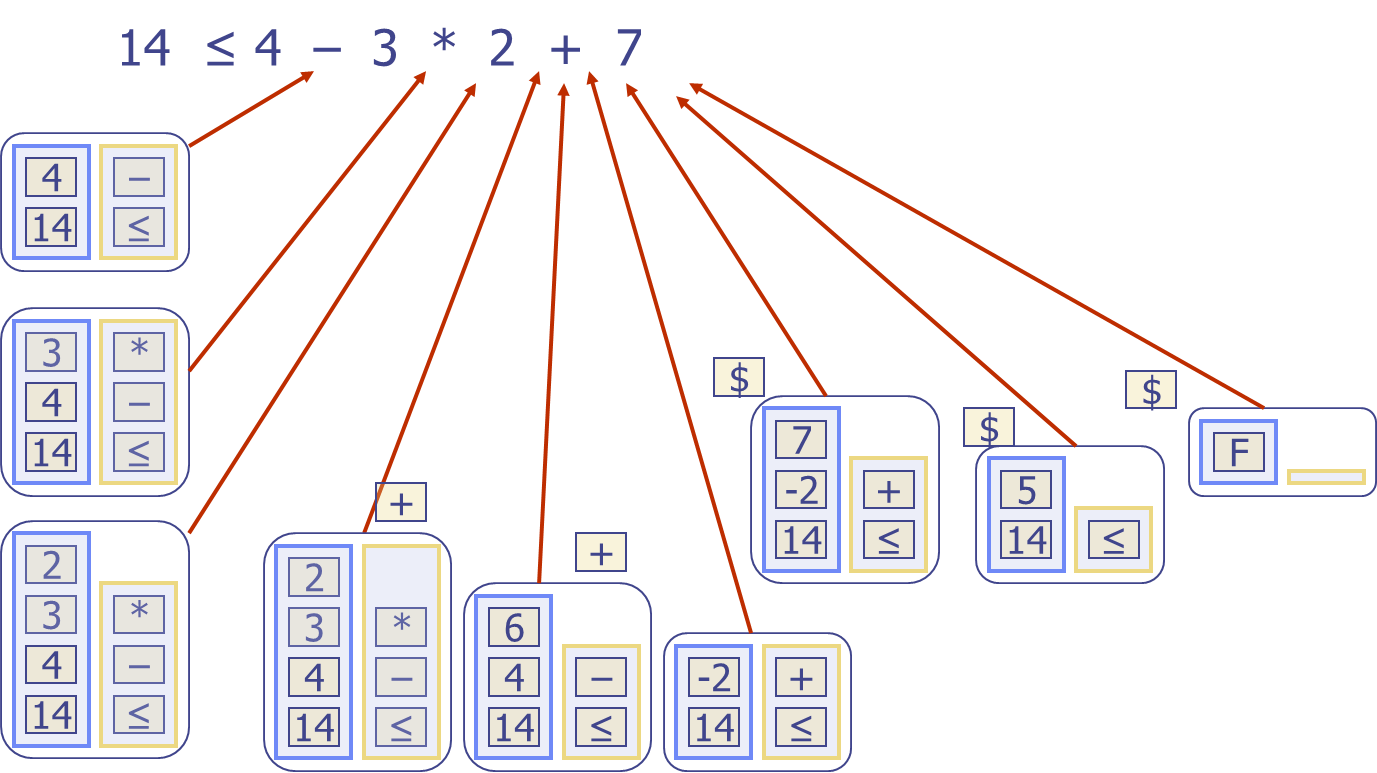
\includegraphics[width=11cm]{asp-05-pic05.png}
  \end{center}
\end{frame}

\section[P: Raspon]{Primer: izačunavanje raspona}
\begin{frame}[fragile]
  \frametitle{Primer: izračunavanje raspona}
  \begin{itemize}
    \item za dati niz $X$, \myred{raspon} $S[i]$ od $X[i]$ najveći broj susednih 
    elemenata $X[j]$ koji neposredno prethode $X[i]$ takvi da je $X[j]\leq X[i]$
    \item primene u finansijskoj analizi 
  \end{itemize}
  \begin{center}
    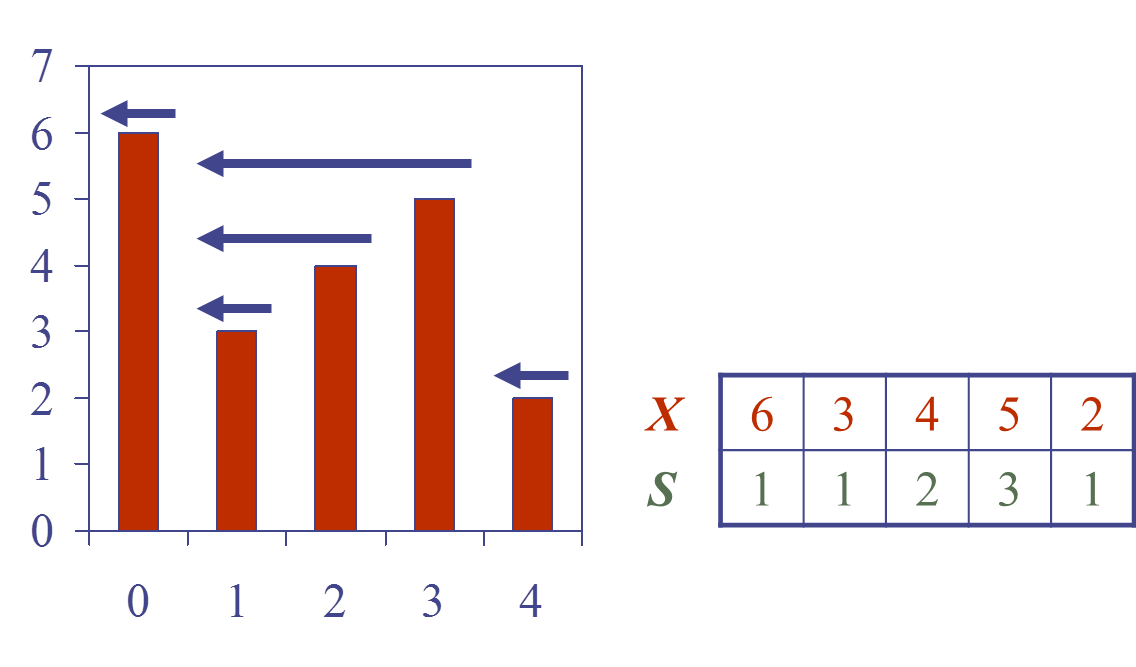
\includegraphics[width=9cm]{asp-05-pic06.png}
  \end{center}
\end{frame}

\begin{frame}[fragile]
  \frametitle{Kvadratni algoritam}
\myred{spans1}($x, n$)
\begin{algorithmic}
\REQUIRE niz $X$ od $n$ celih brojeva
\ENSURE niz $S$ sa rasponima od $X$
\STATE $S \leftarrow$ novi niz od $n$ celih brojeva
\FOR{$i\leftarrow 0$ \TO $n-1$}
  \STATE $s\leftarrow 1$
  \WHILE{$s\leq i \land X[i-s]\leq X[i]$}
    \STATE $s\leftarrow s+1$
  \ENDWHILE
  \STATE $S[i]\leftarrow s$
  \RETURN $S$
\ENDFOR
\end{algorithmic}
\end{frame}

\begin{frame}[fragile]
  \frametitle{Izračunavanje raspona pomoću steka}
  \begin{itemize}
    \item na steku čuvamo indekse elemenata koji su vidljivi kada ,,gledamo unazad``
    \item skeniramo niz s leva u desno
    \item neka je $i$ tekući indeks
    \item skidamo indekse sa steka sve dok ne nađemo indeks $j$ takav da je $X[i]<X[j]$
    \item računamo $S[i]\leftarrow i-j$
    \item stavimo $x$ na stek
  \end{itemize}
  \begin{center}
    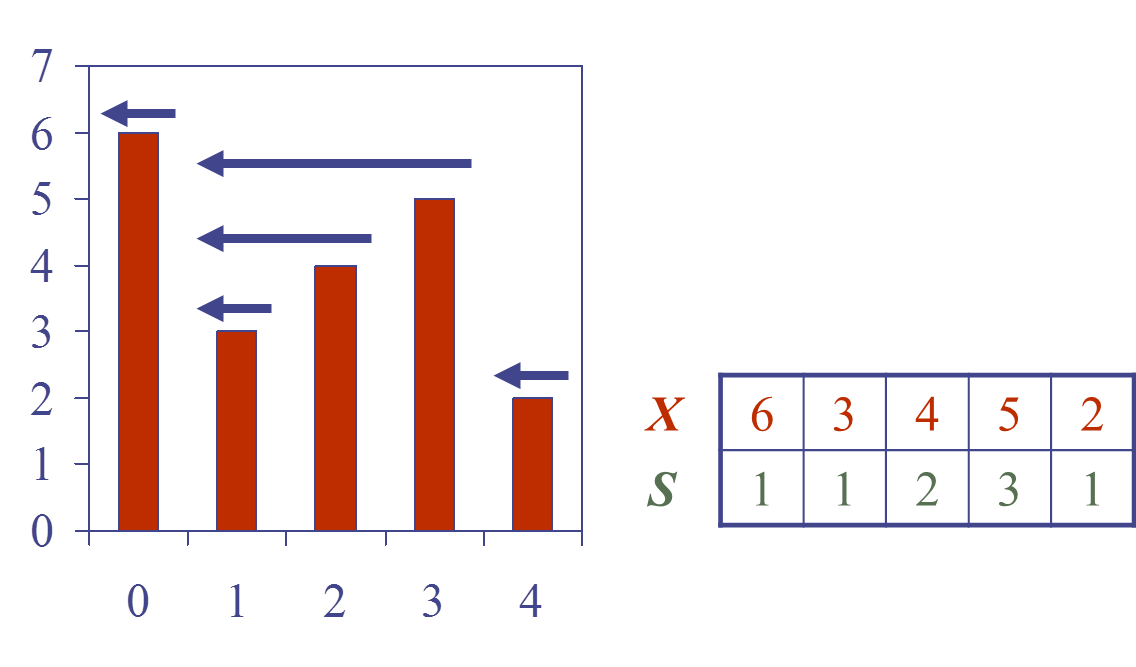
\includegraphics[width=7cm]{asp-05-pic06.png}
  \end{center}
\end{frame}

\begin{frame}[fragile,shrink=5]
  \frametitle{Linearni algoritam}
\myred{spans2}($x, n$)
\begin{algorithmic}
\REQUIRE niz $X$ od $n$ celih brojeva
\ENSURE niz $S$ sa rasponima od $X$
\STATE $S \leftarrow$ novi niz od $n$ celih brojeva
\STATE $A \leftarrow$ novi prazan stek
\FOR{$i\leftarrow 0$ \TO $n-1$}
  \WHILE{$\neg$ $A$.is\_empty()\, $\land\, X$[$A$.top()]$\leq X[i]$}
    \STATE $A$.pop()
  \ENDWHILE
  \IF{$A$.is\_empty()}
    \STATE $S[i]\leftarrow i+1$
  \ELSE
    \STATE $S[i]\leftarrow i-A$.top()
  \ENDIF
  \STATE $A$.push($i$)  
\ENDFOR
\RETURN $S$
\end{algorithmic}
\end{frame}

\begin{frame}[fragile]
  \frametitle{Linearni algoritam}
  \begin{itemize}
    \item svaki indeks u nizu\ldots
    \item \ldots je stavljen na stek tačno jednom
    \item \ldots je skinut sa steka najviše jednom
    \item naredbe u while petlji su izvršene najviše $n$ puta
    \item algoritam radi u $O(n)$ vremenu
  \end{itemize}
\end{frame}

\end{document}
